\chapter{Principe de la solution envisagée}
\label{chap:sol}

  Notre solution est découpée en trois étapes incrémentales. Dans un premier
  temps, nous remettons en place le procédé de migration de processus
  mono-thread. Dans un second temps, nous ajoutons le support du
  multi-thread. Enfin, nous ré-implémentons un composant d'ALMOS appelé DQDT,
  nécessaire pour la politique de migration dans le noyau.

  \begin{paragraph}{Remarque:}
    Dans la section~\ref{sec:mono}, le mot \textit{processus} est utilisé pour
    désigner un processus composé d'un seul thread. Dans la suite de ce
    chapitre, à partir de la section~\ref{sec:multi}, on considère que les
    processus ont plusieurs threads.
  \end{paragraph}


  \section{Support des processus mono-thread}
  \label{sec:mono}

    Cette première étape a pour but de mettre en place deux mécanismes:
    \benumline \item la migration de processus entre noyaux \item la création
    distante de processus\eenumline. Pour compléter ces deux objectifs, il est
    nécessaire de définir l'ensemble des structures partagées par les processus
    et lesquelles doivent nécessairement être maintenues cohérentes tout au long
    de l'exécution.

    \subsection{Principes}

      \subsubsection{Rappels}

        L'appel système \texttt{fork()} est usuellement utilisé pour créer un
        processus dans un système. Lorsqu'un processus fait appel à cette
        fonction, un processus identique à l'appelant est créé. L'appelant est
        nommé \textit{père}, et le résultat est appelé \textit{fils}. Le fils
        étant une copie de son père, son exécution commence juste après l'appel
        système \texttt{fork()}.

        Pour qu'un fils exécute un autre programme que celui du père, il faut
        utiliser l'appel système \texttt{exec()}. C'est lui qui permet de
        remplacer le code exécuté par un processus.\\

        Dans la très grande majorité des cas, un appel à \texttt{fork()} est
        suivit d'un appel à \texttt{exec()}. C'est la principale manière de
        lancer des applications différentes dans un système\footnote{Voir
          \texttt{posix\_spawn()} pour une alternative.}. Un exemple
          d'utilisation de ces deux fonctions est donné par le
          Listing~\ref{lst:fork-exec}.

        \lstinputlisting[label={lst:fork-exec}, caption=Utilisation de
          \texttt{fork()/exec()}. La valeur de retour de \texttt{fork()} permet
          de différencier si le processus en cours d'exécution est le père ou le
          fils.]{include/code/example.c} \FloatBarrier

      \subsubsection{Migration}

        La migration de processus repose sur le mécanisme des RPC du
        noyau. Cette opération consiste à déplacer un processus dans un nouveau
        noyau pendant son exécution. Pour déplacer un processus, il faut envoyer
        les informations nécessaires au noyau destinataire afin qu'il puisse
        reconstruire l'espace virtuel du processus. On a notamment besoin des
        adresses de début et de fin:
        \begin{itemize}
          \item de la pile utilisateur
          \item du tas
          \item du code
          \item des arguments
          \item des données
        \end{itemize}
        Pour l'identification et l'exécution, il faut envoyer les informations
        suivantes:
        \begin{itemize}
          \item le \texttt{pid}
          \item l'identifiant du noyau d'origine
          \item le \texttt{pid} sur le noyau d'origine
          \item l'identificateur de groupe
          \item la priorité
          \item la politique d'ordonnancement\\
        \end{itemize}

        La migration n'est pas explicite pour le programmeur. Elle est à
        l'appréciation de la DQDT, présentée en section~\ref{sec:dqdt}. On veut
        simplement ici mettre en place un mécanisme via RPC permettant de migrer
        un processus à n'importe quel moment de son exécution.

      \subsubsection{Création distante}

        Migrer un processus pendant sa création, donc lors du \texttt{fork()},
        est une hypothèse que nous avons écartée. En effet, après avoir déplacé
        toutes les données du fils sur le nouveau noyau, la probabilité que ce
        dernier fasse un \texttt{exec()} est très grande. Par cet appel, il
        écrase toutes les données que l'on a déplacées juste avant. On paye donc
        le coût de la migration inutilement.\\

        Pour implémenter ce mécanisme, nous avons choisi de nous baser sur
        l'appel système \texttt{exec()}. Nous allons le modifier en ajoutant un
        appel aux fonctions de la DQDT. Si en retour le noyau s'aperçoit que le
        processus doit être migré, alors les informations citées précédemment
        seront envoyées. Ici, les données les plus importantes à transmettre
        sont le chemin vers l'exécutable et les arguments spécifiés dans l'appel
        \texttt{exec()} (voir l'algorithme~\ref{lst:fork-exec}). En effet, on
        veut que le processus qui sera créé exécute un nouveau code et pas celui
        de son père.\\

        Attendre un appel à \texttt{exec()} pour effectuer la migration permet
        de ne pas briser la localité spatiale des processus ayant un lien de
        parenté, et qui par définition accèdent aux mêmes données. On pense par
        exemple au navigateur web Firefox, qui gère ses onglets en utilisant un
        processus complet et non plus un thread~\citep{mozillaElectrolysis}.\\

        On note qu'un processus qui crée beaucoup de fils sans faire d'appel à
        \texttt{exec()} ne représente pas une menace pour la stabilité du
        système. En effet, au bout d'un temps $T$ borné, la DQDT verra la
        surchage engendrée par tous ces processus. Les mécanismes de migration
        expliqués précédemment seront alors activés.

        \begin{paragraph}{Remarque:}
          Un appel à \texttt{exec()} ne migre pas forcément un processus. La
          migration se fait selon la politique de la DQDT.
        \end{paragraph}


    \subsection{Maintien de cohérence}

      Comme nous l'avons vu précédemment, ces deux opérations représentent un
      enjeu quant aux structures de données que contiennent les processus, en
      particulier celles qu'ils partagent:
      \begin{itemize}
      \item les descripteurs de fichiers ouverts
      \item les zones mémoires partagées
      \end{itemize}

      Les descripteurs de fichiers contiennent des données qui doivent être
      maintenues cohérentes\footnote{C'est une obligation de la norme
        POSIX~\citep{posix2013} que le noyau ALMOS a choisi de respecter.}. Ces
      informations sont l'offset et le compteur de référence. Le premier indique
      la position à laquelle se trouve le processus dans un fichier. Le second
      permet de savoir combien de processus ont ouvert le même fichier.

      \begin{paragraph}{Remarque:}
        Cette cohérence s'applique également dans le cadre d'un processus ayant
        plusieurs threads : chaque action de l'un doit être visible des
        autres.\\
      \end{paragraph}

      Lorsqu'un processus ouvre un fichier puis crée un fils, les modifications
      du père doivent être visibles pour le fils, et inversement. Or, chaque
      modification déplace la tête de lecture. Afin de maintenir la cohérence
      dans le fichier, la valeur de l'offset doit être la même pour tous les
      processus ayant ouvert le fichier.

      Dans les sytèmes UNIX, chaque processus à son espace virtuel et ne peut
      pas accéder à celui des autres. Néanmoins, les noyaux permettent d'allouer
      de la mémoire en mode \texttt{SHARED}. Ainsi, deux processus peuvent se
      partager une certaine zone mémoire et ainsi échanger des
      informations. Pour des raisons évidentes, le contenu de ces zones mémoires
      doit impérativement être cohérent\footnote{On ne parle pas de la structure
        représentant la zone mémoire, qui elle est propre aux processus.}.


    \subsection{Accélération de la migration}

      Afin de faciliter le maintien de la cohérence et surtout d'accélérer la
      migration, nous devons redéfinir l'implémentation des descripteurs de
      fichiers et des zones mémoires. Il est nécessaire d'éliminer l'utilisation
      des pointeurs qui deviennent faux lorsqu'un processus change de noyau. En
      effet, une adresse dans un noyau $N$ n'est pas significative dans un noyau
      $N'$. Un exemple pour illustrer cela est celui des processus
      père/fils. Chaque processus doit savoir qui est son père, et possède un
      pointeur en direction de la \texttt{struct task} de ce dernier. Si le fils
      est migré sur un nouveau noyau, cette adresse n'est plus valable.

      Nous devons donc réduire au maximum le nombre de pointeurs, et notamment
      ceux utilisés pour gérer les descripteurs de fichiers ouverts ainsi que
      les zones de mémoire virtuelle d'un processus. Supprimer ces pointeurs
      implique de devoir changer l'implémentation de la structure de données
      utilisée pour stocker toutes les informations. Nous devons utiliser des
      tableaux pour enregistrer les informations sur les fichiers ouverts par
      les processus. Ces tableaux sont plus faciles à migrer puisqu'il s'agit
      simplement d'en faire une copie dans la mémoire du noyau destinataire.

      Nous avons actuellement deux solutions à l'étude:
      \begin{itemize}
        \item utiliser une table de hachage par calcul
        \item utiliser une table de hachage chainée
      \end{itemize}

      Aucune n'a pour l'instant été choisie. Néanmoins, quelque soit la solution
      envisagée, les entrées et sorties sont similaires, ce qui nous permet de
      n'effectuer qu'une seule spécification. Nous allons utiliser l'adresse
      virtuelle accédée comme entrée de la fonction de hash. En sortie, nous
      obtenons l'adresse physique de la région virtuelle associée.

      \begin{center}
        \texttt{hash(v\_addr) = v\_reg\_addr}
      \end{center}

      La première solution nous garantie de n'avoir qu'une table à
      gérer. Néanmoins, cette gestion est assez difficile à implémenter. À
      l'inverse, la table de hash chainée est plus simple à mettre en \oe uvre
      mais les indirections que nous pensons utiliser en feront un objet plus
      complexe que la précédente solution. Ces deux possibilités n'ont pour
      l'instant pas été estimées en terme de coût pour le système. Elles restent
      donc à l'état d'hypothèse jusqu'à ce que l'une d'elle s'avère plus
      efficace.


  \section{Ajout du multi-thread}
  \label{sec:multi}  

    Une fois le support des processus mono-thread en place, nous devons ajouter
    le support du multi-thread. Cette opération s'avère très délicate, et
    représente probablement l'étape la plus compliquée de ce stage.\\

    Dans la section~\ref{sec:mono}, nous avons parlé des structures de données
    critiques pour les processus mono-thread. Nous allons à présent nous
    intéresser aux processus multi-thread. Après étude du problème, nous avons
    principalement deux structures qui posent problème (en plus de celle vues en
    ~\ref{sec:mono}):
    \begin{itemize}
      \item la table des pages
      \item les signaux
    \end{itemize}  

    \subsection{La table des pages}

      La table des pages est la structure de données des processus permettant
      les traductions des adresses virtuelles en adresses physiques. Chaque
      processus possède sa propre table des pages, et tous les threads d'un
      processus accèdent à cette table.

      Le problème de cette structure sont les accès fréquents lors des miss TLB
      (le cache de traduction d'adresses virtuelles $\leftrightarrow$
      physiques). Si l'on migre un thread du processus sur un autre noyau, ce
      dernier accèdera par passage de messages à la table, ce qui n'est pas
      envisageable pour des raisons de performances. Il faut donc copier la
      table des pages entièrement, ce qui n'est pas gratuit, et maintenir
      ensuite une cohérence entre toutes les tables répliquées dans les
      clusters. En prenant en compte le fait que chaque processus possède une
      table de page, les surcoûts liés aux communications apparaîssent
      rapidement.

      Pour répondre à cette problématique, nous allons intégrer le concept des
      processus hybrides~\citep{almaless2014universite}. Un processus hybride
      contient des threads qui ont leur propre espace virtuel qui n'est plus
      accessible par les autres threads du processus. Le noyau maintient
      néanmoins la cohérence entre ces espaces. De plus, chaque thread possède
      sa table des pages, qui contient des pages communes avec les autres
      threads du processus, mais également ses propres pages locales. Le
      mécanisme proposé est illustré par la figure~\ref{fig:almos-page-table}.

      \begin{figure}[ht]
        \centering
        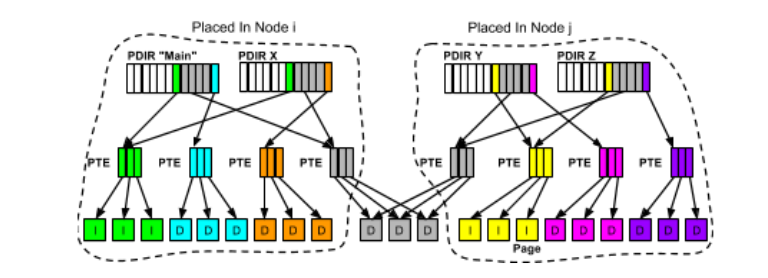
\includegraphics[width=\textwidth]{almos-page-table}
        \caption{Organisation de la table des pages pour quatre threads d'un
          même processus. Deux threads sont placés sur un cluster $i$, et deux
          sur un cluster $j$. Les threads partagent certaines pages de données
          et d'instructions, parfois entre clusters, mais ont également leurs
          pages privées~\citep{almaless2014universite}.}
        \label{fig:almos-page-table}
      \end{figure}

      L'intérêt des processus hybrides est double:

      \begin{itemize}
        \item on évite le goulot d'étranglement sur la table des pages
        \item les espaces virtuels des threads ne sont plus stockés dans le
          processus mais sont indépendants, on a donc économisé de la place dans
          la mémoire virtuelle du processus
      \end{itemize}

      Cette solution permet de minimiser le coût de la cohérence des tables
      entre tous les réplicas et permet également d'alléger les accès
      atomiques. En effet, une application massivement parallèle minimisera les
      dépendances de données entres threads, et donc les pages communes.\\

      Par manque de temps, ce concept n'a pas été implémenté dans le noyau
      ALMOS. Nous allons donc devoir le mettre en place, avec dans un premier
      temps l'objectif d'avoir une table des pages distribuée entre les
      threads.


    \subsection{Les signaux}

      Dans cette partie, nous allons devoir mettre en place des mécanismes pour
      la transmission des signaux lorsque les threads sont distribués sur
      plusieurs noyaux. En effet, la norme POSIX stipule que la portée des
      signaux est un processus dans son ensemble~\citep{man2015signal}.

      Pour cela, il faudra redéfinir la notion de \texttt{pid}. Un \texttt{pid}
      sera découpé en deux parties \benumline \item la partie haute indiquera la
      valeur du cluster sur lequel s'exécute le thread \item la partie basse
      donnera la valeur classique du \texttt{pid} sur ce
      cluster\eenumline. L'application d'un masque sur le champ \texttt{pid}
      permettra alors d'obtenir l'information souhaitée.

      Enfin, après une migration, un processus enverra sa nouvelle adresse au
      noyau d'origine, qui le modifiera dans sa table des processus. Ainsi, le
      noyau d'origine des processus connait en permanence la localisation de ses
      fils sur la machine. Ce mécanisme nous permet de pouvoir transmettre les
      signaux.


  \section{La DQDT}
  \label{sec:dqdt}

    Cette partie du stage est ``optionnelle''. La ré-implémentation de ce
    composant est un besoin réel pour ALMOS, néanmoins cela implique que les
    étapes présentées précédemment soient finalisées.

    La DQDT, pour \textit{Distributed Quaternary Decision Tree}, est le
    composant d'ALMOS assurant une vision cohérente et temps-réel\footnote{C'est
      un abus de langage qui est fait ici. Nous voulons simplement montrer que
      la DQDT permet d'avoir en permanence les taux d'utilisation des 4096
      processeurs de la plateforme.} de l'utilisation des ressources. Dans la
    version de Ghassan~\citet{almaless2014universite}, la DQDT repose sur des
    serveurs répliqués dans tous les clusters. Chaque cluster physique
    représente une feuille de la DQDT. Ces serveurs récupèrent les informations
    sur l'occupation de la machine (c\oe urs et mémoire), et calculent une
    moyenne d'utilisation pour chaque cluster. Cette information est stockée
    dans un n\oe ud de l'arbre. Chaque étage de l'arbre représente un niveau
    d'abstraction. Comme le montre la figure~\ref{fig:dqdt-logical}, le premier
    niveau, en noir, est celui des clusters physiques. Le second niveau, en
    bleu, regroupe 4 clusters. C'est un cluster logique de niveau 1. Le dernier,
    en rouge, regroupe quatre clusters logiques de niveau 1 dans un cluster
    logique de niveau 2. Ces niveaux sont matérialisés par les étages de
    l'arbre, comme le montre la figure~\ref{fig:dqdt-tree}.\\

    \begin{figure}[ht]
      \begin{subfigure}[b]{0.5\textwidth}
        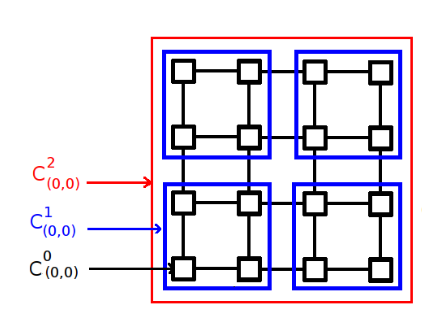
\includegraphics[scale=0.4]{dqdt-logical}
        \caption{Découpage de la plateforme}
        \label{fig:dqdt-logical}
      \end{subfigure}
      \begin{subfigure}[b]{0.4\textwidth}
        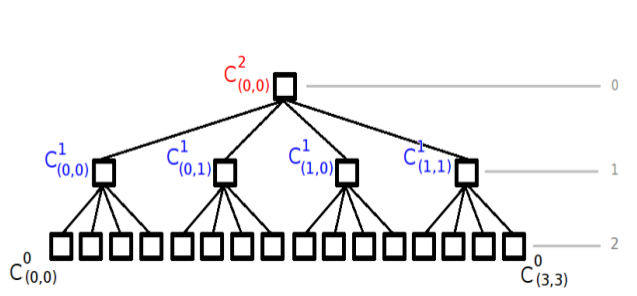
\includegraphics[scale=0.4]{dqdt-tree}
        \caption{Représentation du découpage}
        \label{fig:dqdt-tree}
      \end{subfigure}
      \caption{Construction de la DQDT~\citep{almaless2014universite}.}
    \end{figure}

    La DQDT, comme la plupart des composants noyaux d'ALMOS, repose sur le
    mécanisme de la mémoire virtuelle répartie entre les clusters. Si l'on
    change ALMOS en multi-noyau, les serveurs de la DQDT ne peuvent plus
    communiquer grâce à la mémoire virtuelle. Ils sont obligés d'utiliser le
    passage de messages entre les noyaux.

    Notre but est de changer le schéma de communication de la DQDT. Deux
    techniques peuvent être utilisées:
    \begin{itemize}
      \item avoir une solution portable sur n'importe quelle architecture
        matérielle : nous utilisons le passage de messages
      \item avoir une solution efficace sur l'architecture TSAR : nous profitons
        de mécanismes matériels nous permettant d'accéder directement à la
        mémoire physique des clusters voisins.
    \end{itemize}

    Nous allons dans un premier temps implémenter une version efficace sur TSAR,
    puis selon le temps restant, une solution générique.


    \nomenclature{DQDT}{Distributed Quaternary Decision Tree}
    \nomenclature{RPC}{Remote Procedure Call}
    \nomenclature{UNIX}{Uniplexed Information and Computing Service}
    \nomenclature{PDIR}{Page DIRectory}
    \nomenclature{PTE}{Page Table Entry}
